\documentclass[11pt]{article}
\usepackage[utf8]{inputenc}
\usepackage{amsmath}
\usepackage{amssymb}
\usepackage{algpseudocode}
\usepackage{listings}
\usepackage{xcolor}
\usepackage{booktabs}
\usepackage{multirow}
\usepackage{graphicx}
\usepackage{hyperref}
\usepackage{geometry}
\usepackage{titlesec}
\usepackage{enumitem}
\usepackage{booktabs}
\usepackage{forest}
\usepackage{tikz}
\usepackage{float} 
\usepackage{longtable}
\usepackage{import} 
\usepackage[ruled,vlined]{algorithm2e}
\usetikzlibrary{calc, positioning, arrows.meta}
\geometry{a4paper, margin=1in}
\titleformat{\section}{\large\bfseries}{\thesection}{1em}{}
\titleformat{\subsection}{\normalsize\bfseries}{\thesubsection}{1em}{}

\definecolor{codegreen}{rgb}{0,0.6,0}
\definecolor{codegray}{rgb}{0.5,0.5,0.5}
\definecolor{codepurple}{rgb}{0.58,0,0.82}
\definecolor{backcolour}{rgb}{0.95,0.95,0.92}

\lstset{
    language=C++,
    backgroundcolor=\color{backcolour},   
    commentstyle=\color{codegreen},
    keywordstyle=\color{magenta},
    numberstyle=\tiny\color{codegray},
    stringstyle=\color{codepurple},
    basicstyle=\ttfamily\footnotesize,
    breakatwhitespace=false,         
    breaklines=true,                 
    captionpos=b,                    
    keepspaces=true,                 
    numbers=left,                    
    numbersep=5pt,                  
    showspaces=false,                
    showstringspaces=false,
    showtabs=false,                  
    tabsize=4,
    frame=lines,
}

\begin{document}

\begin{center}
    \centering
    {\Huge \textbf{CSC3060 Project 4 Report}} \\[0.5cm]
    
    \textbf{Student Name} \quad Chaoyi, Sun \\[0.1cm]
    \textbf{Student ID} \quad 124090550 \\[1cm]
\end{center}

\section{Implementation Summary}
\subsection{Task1}

Task 1 requires the implementation of core access logic and fundamental mechanisms for a single-level L1 cache simulator. The completed implementation consists of three core components: address decomposition, cache access logic, and the baseline replacement policy.

\begin{itemize}
\item \textbf{Address Decomposition and Reconstruction} \\
Based on the provided cache geometry, including cache size, associativity, and block size. Bitwise shift and masking operations are employed to accurately extract the set index and tag from a 64-bit memory address.

\item\textbf{Cache Access Logic}\\
For a cache access request, if a matching tag is found in the target set, the metadata of the hit line is updated; otherwise, the requested block is installed into an empty invalid line if one is available, or a victim block is selected by the replacement policy for eviction when the set is full.

\item\textbf{LRU Replacement Policy} \\
Uses timestamps to track access order. On replacement, selects the cache line with the earliest timestamp as the victim.
\end{itemize}

\subsection{Task2}

Task 2 involves the integration of an L2 cache and the construction of a multi level memory hierarchy where L1, L2, and Main Memory are connected in sequence.

\begin{itemize}
\item \textbf{Hierarchy Hookup} \\
When the \texttt{--enable-l2} flag is active, an L2 cache is instantiated and positioned between L1 and Main Memory. The \texttt{next\_level} pointer of L1 is updated to point to L2, creating a chain where L1 misses are forwarded to the secondary cache rather than directly to Main Memory.

\item \textbf{Recursive Miss Path} \\
L1 misses trigger a search in L2, and Main Memory is accessed only after an L2 miss. This hierarchy reduces total cycles by serving a significant portion of L1 misses at a lower L2 latency.

\item \textbf{Write Back Propagation} \\
Dirty blocks evicted from L1 are written into L2. If those blocks are subsequently evicted from L2, the modified data is propagated to Main Memory to maintain consistency across the entire hierarchy.
\end{itemize}

\subsection{Task3}

Task 3 optimizes the cache simulator with advanced replacement policies and prefetching mechanisms to minimize AMAT on a personalized trace.

\begin{itemize}
\item \textbf{Advanced Replacement Policies} \\
SRRIP assigns a re-reference priority value to each cache line, while BIP inserts most new lines with low priority. Both policies effectively resist scan-induced cache pollution.

\item \textbf{Prefetching Strategies} \\
NextLine prefetches the subsequent cache block on each access. Stride detects repeating access patterns and prefetches future blocks at the computed stride once the pattern is confirmed.

\item \textbf{Prefetch Integration} \\
Prefetching is triggered by demand requests to load predicted blocks into the cache as clean entries. Successful prefetches are promoted to standard lines upon a subsequent hit, allowing the replacement policy to recognize and prioritize useful data.
\end{itemize}

\section{Address Mapping Explanation}
\subsection{Calculation Methods}
Given a cache configuration with total size $C$ (in KB), associativity $E$, and block size $B$ (in bytes). Let $S = \dfrac{1024C}{BE}$ be the number of sets in the cache.

\begin{center}
    \begin{minipage}[c]{0.45\textwidth}
        \centering
        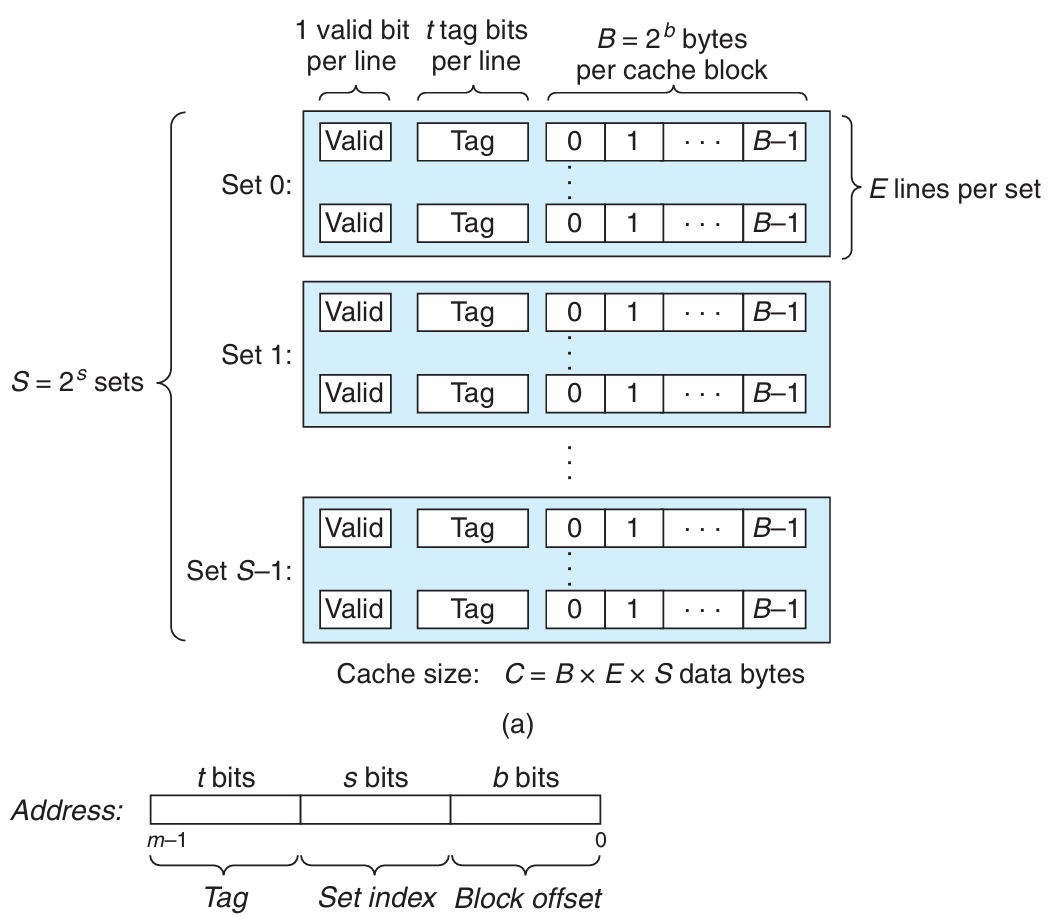
\includegraphics[width=\textwidth]{img/address mapping.png}
    \end{minipage}
    \hfill
    \begin{minipage}[c]{0.45\textwidth}
        \centering
        \begin{tabular}{|l|l|}
            \hline
            \textbf{Parameter} & \textbf{Formula} \\
            \hline
            Block offset bits & $\log_2 B$ \\
            \hline
            Set index bits & $\log_2 S$ \\
            \hline
            Tag bits & $64 - \log_2 B - \log_2 S$ \\
            \hline
        \end{tabular}
    \end{minipage}
\end{center}

\subsection{Impact of Cache Geometry Changes}
\begin{itemize}
    \item Increasing block size increases offset bits but decreases index bits while leaving tag bits unchanged.
    \item Increasing cache size increases index bits and decreases tag bits.
    \item Increasing associativity decreases index bits and increases tag bits.
\end{itemize}

\begin{table}[h]
\centering
\begin{tabular}{|l|l|l|l|}
\hline
\textbf{Change} & \textbf{Block Offset Bits} & \textbf{Set Index Bits} & \textbf{Tag Bits} \\
\hline
Increase block size $B$ & $\uparrow$ & $\downarrow$ & — \\
\hline
Increase cache size $S$ & — & $\uparrow$ & $\downarrow$ \\
\hline
Increase associativity $E$ & — & $\downarrow$ & $\uparrow$ \\
\hline
\end{tabular}
\end{table}

\section{Task 1 Testing}
\subsection{Testing Methodology}
The simulator was tested on \texttt{trace\_sanity.txt} using diverse cache geometries including various sizes, associativity levels, and block sizes. These tests confirmed that the dynamic address decomposition and LRU policy correctly handle frequent misses in small configurations as well as corner cases like direct-mapped caches. All output metrics such as hit rate, write-back counts, and AMAT were cross-checked against reference results to ensure the absolute accuracy of the core access logic.
\subsection{Test Configurations}

\begin{table}[h!]
\centering
\resizebox{\textwidth}{!}{
\begin{tabular}{|l|c|c|c|c|c|c|c|c|}
\hline
\textbf{Test Category} & \textbf{L1 Size} & \textbf{Assoc} & \textbf{Block} & \textbf{Hit Rate} & \textbf{Misses} & \textbf{WB} & \textbf{Mem Acc} & \textbf{AMAT} \\ \hline
\multirow{3}{*}{Basic Configs} & 16 KB & 4 & 64 B & 21.43\% & 44 & 6 & 50 & 79.57 \\
                               & 32 KB & 4 & 32 B & 21.43\% & 44 & 2 & 46 & 79.57 \\
                               & 64 KB & 8 & 128 B & 60.71\% & 22 & 0 & 22 & 40.29 \\ \hline
Direct Mapped    & 32 KB & 1 & 64 B & 42.86\% & 32 & 2 & 34 & 58.14 \\ \hline
High Associativity & 64 KB & 32 & 64 B & 58.93\% & 23 & 0 & 23 & 42.07 \\ \hline
Large Capacity   & 128 KB & 4 & 64 B & 62.50\% & 21 & 0 & 21 & 38.50 \\ \hline
Minimum Capacity & 1 KB & 2 & 64 B & 21.43\% & 44 & 8 & 52 & 79.57 \\ \hline
\end{tabular}
}
\end{table}

\section{Task 2 Hierarchy Explanation}
\subsection{L1, L2, and Memory Interaction}
\usetikzlibrary{positioning, arrows.meta, shapes.geometric}

\begin{figure}[h]
\centering
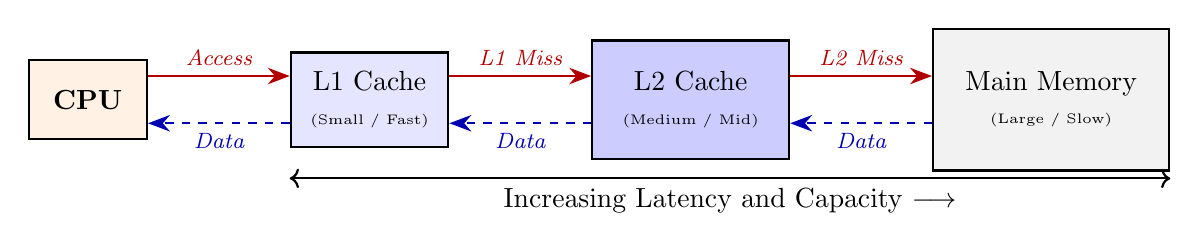
\begin{tikzpicture}[
    node distance=1.2cm and 1.8cm,
    cpu/.style={rectangle, draw, thick, fill=orange!10, minimum width=1.5cm, minimum height=1cm, font=\bfseries},
    l1/.style={rectangle, draw, thick, fill=blue!10, minimum width=2.0cm, minimum height=1.2cm, align=center},
    l2/.style={rectangle, draw, thick, fill=blue!20, minimum width=2.5cm, minimum height=1.5cm, align=center},
    mem/.style={rectangle, draw, thick, fill=gray!10, minimum width=3.0cm, minimum height=1.8cm, align=center},
    arrow_fwd/.style={-{Stealth[scale=1.2]}, thick, color=red!70!black},
    arrow_back/.style={-{Stealth[scale=1.2]}, thick, dashed, color=blue!70!black},
    label_style/.style={font=\footnotesize\itshape}
]

\node[cpu] (cpu) {CPU};
\node[l1, right=of cpu] (l1) {L1 Cache \\ \tiny (Small / Fast)};
\node[l2, right=of l1] (l2) {L2 Cache \\ \tiny (Medium / Mid)};
\node[mem, right=of l2] (mem) {Main Memory \\ \tiny (Large / Slow)};

\draw[arrow_fwd] ([yshift=3mm]cpu.east) -- ([yshift=3mm]l1.west) 
    node[midway, above, label_style] {Access};
\draw[arrow_fwd] ([yshift=3mm]l1.east) -- ([yshift=3mm]l2.west) 
    node[midway, above, label_style] {L1 Miss};
\draw[arrow_fwd] ([yshift=3mm]l2.east) -- ([yshift=3mm]mem.west) 
    node[midway, above, label_style] {L2 Miss};

\draw[arrow_back] ([yshift=-3mm]mem.west) -- ([yshift=-3mm]l2.east) 
    node[midway, below, label_style] {Data};
\draw[arrow_back] ([yshift=-3mm]l2.west) -- ([yshift=-3mm]l1.east) 
    node[midway, below, label_style] {Data};
\draw[arrow_back] ([yshift=-3mm]l1.west) -- ([yshift=-3mm]cpu.east) 
    node[midway, below, label_style] {Data};

\draw[thick, <->] ([yshift=-1cm]l1.west) -- ([yshift=-1cm]mem.east) 
    node[midway, below] {Increasing Latency and Capacity $\longrightarrow$};

\end{tikzpicture}
\end{figure}
\noindent As illustrated in the figure, memory requests originate at the CPU and traverse the hierarchy toward Main Memory. A hit at any cache level triggers an immediate data return along the response path. In the case of an L1 miss, the request is forwarded to L2, and a subsequent L2 miss results in a Main Memory access. Once the data is retrieved, it flows back through each level to satisfy the CPU request. Simultaneously, dirty victims follow an eviction path where L1 writes back modified data to L2, and L2 propagates its own dirty blocks to Main Memory to maintain data consistency.
\subsection{Impact of L2 on System Performance}

\begin{itemize}
\item \textbf{Filtering of Main Memory Traffic} \\
Main memory accesses dropped from 46 to 23 in the reference trace. This reduction occurs because the L2 cache acts as a secondary filtering layer. Every L1 miss that results in an L2 hit is successfully served within the cache hierarchy, preventing a high latency request from reaching Main Memory.

\textbf{Average Memory Access Time Optimization} \
AMAT decreased from 79.57 to 45.21 cycles. Although L1 misses now incur additional L2 access latency, this overhead is negligible compared to the much higher memory penalty that L2 helps avoid. With L2 capturing 50\% of L1 misses, the average data access time is significantly reduced.
\item \textbf{Write Back Staging and Buffer Effect} \\
The write back process is now staged between levels. Dirty evicts from L1 are written into L2 instead of directly to Main Memory. This creates a buffer effect where modified data can stay within the faster cache hierarchy for a longer duration.
\end{itemize}
\section{Task 3 Design Choices}

\subsection{Replacement Policies}

Three replacement policies are implemented: LRU, SRRIP, and BIP. LRU serves as the baseline. SRRIP assigns a re-reference priority value to each cache line, protecting hot data from scan-induced pollution. BIP is implemented but not used in the final configuration, as SRRIP provides better protection for the trace's mixed phase behavior.

\subsection{Prefetchers}

Three prefetchers are implemented: NextLine, Stride, and a custom prefetcher. NextLine prefetches the subsequent cache block, benefiting sequential patterns. Stride detects repeating strides and prefetches future blocks once the pattern is confirmed.
\newline
The custom prefetcher is designed based on the personalized trace. Analysis reveals that certain strides dominate the access pattern. Therefore, when such strides are detected, the custom prefetcher issues an additional prefetch to further reduce miss penalty.
\section{Trace Analysis}

\subsection{Trace Generation}

The personalized trace was generated using student ID \textbf{124090550} as the seed:
\begin{verbatim}
./trace_generator/workload_gen student 124090550 > my_trace.txt
\end{verbatim}

\subsection{Access Patterns}

The trace was analyzed using the provided \texttt{trace\_analyzer.py} script with a block size of 64 bytes. 
\begin{table}[h]
\centering
\begin{tabular}{|l|l|l|}
\hline
\textbf{Feature} & \textbf{Value} & \textbf{Implication} \\
\hline
Dominant Strides & 7 (45\%), 1 (25\%), 64 (17\%) & Use Stride prefetcher for L1 \\
\hline
Hotspot Set & Set 0 (22.65\% of accesses) & Use high associativity (32-way) \\
\hline
Phase Behavior & Stable loop [2560,4352): 14 blocks, 1 set & Use SRRIP to protect hot data \\
\hline
L1 Miss Pattern & Scan phases: sequential new blocks & Use NextLine prefetcher for L2 \\
\hline
\end{tabular}
\end{table}
\newline
Based on these observations, stride 7 (45\%), stride 1 (25\%), and stride 64 (17\%) together guided the use of Stride prefetcher in L1. The hotspot on set 0 (22.65\%) demanded 32-way associativity. The stable loop phase (14 blocks, 1 set) required SRRIP in L2 to protect hot data from scan pollution. Sequential L1 misses during scan phases made NextLine prefetcher effective for L2.

\section{Experimental Results}


\scriptsize

\begin{table}[H]
\centering
\caption{\small Single-Level L1 Performance Comparison (32KB, 8-way)}
\label{tab:l1_comparison}
\small
\begin{tabular}{llcc}
\toprule
\textbf{Policy} & \textbf{Prefetcher} & \textbf{L1 Hit Rate} & \textbf{AMAT (cycles)} \\
\midrule
\multirow{3}{*}{LRU} & None & 16.17\% & 84.83 \\
                     & NextLine & 74.98\% & 26.02 \\
                     & Stride & 86.66\% & 14.34 \\
\midrule
\multirow{3}{*}{SRRIP} & None & 20.83\% & 80.17 \\
                       & NextLine & 69.32\% & 31.68 \\
                       & Stride & 88.20\% & \textbf{12.80} \\
\midrule
\multirow{3}{*}{BIP} & None & 28.20\% & 72.80 \\
                     & NextLine & 43.42\% & 57.58 \\
                     & Stride & 88.05\% & 12.95 \\
\bottomrule
\end{tabular}
\end{table}

\begin{longtable}{llllccc}
\caption{Full Comparison of Cache Configurations (32KB, 8-way)} \label{tab:full_results} \\
\toprule
\textbf{L1 Policy} & \textbf{L1 Pref.} & \textbf{L2 Policy} & \textbf{L2 Pref.} & \textbf{L1 Hit\%} & \textbf{L2 Hit\%} & \textbf{AMAT} \\ \midrule
\endfirsthead

\multicolumn{7}{c}%
{{\bfseries \tablename\ \thetable{} -- Continued}} \\
\toprule
\textbf{L1 Policy} & \textbf{L1 Pref.} & \textbf{L2 Policy} & \textbf{L2 Pref.} & \textbf{L1 Hit\%} & \textbf{L2 Hit\%} & \textbf{AMAT} \\ \midrule
\endhead

\midrule
\multicolumn{7}{r}{{Continued on next page}} \\
\endfoot

\bottomrule
\endlastfoot

% === Group: LRU+NextLine ===
\multirow{6}{*}{LRU} & \multirow{6}{*}{NextLine} & \multirow{3}{*}{LRU} & NextLine & 74.98\% & 98.07\% & 4.18 \\
 & & & Stride & 74.98\% & 94.96\% & 4.18 \\
 & & \multirow{3}{*}{SRRIP} & NextLine & 74.98\% & 98.06\% & 4.18 \\
 & & & Stride & 74.98\% & 94.78\% & 4.33 \\
 & & \multirow{3}{*}{BIP} & NextLine & 74.98\% & 98.03\% & 4.18 \\
 & & & Stride & 74.98\% & 94.80\% & 4.34 \\ \midrule

% === Group: LRU+Stride ===
\multirow{6}{*}{LRU} & \multirow{6}{*}{Stride} & \multirow{3}{*}{LRU} & NextLine & 86.66\% & 97.54\% & 1.85 \\
 & & & Stride & 86.66\% & 98.07\% & 2.14 \\
 & & \multirow{3}{*}{SRRIP} & NextLine & 86.66\% & 97.53\% & 1.86 \\
 & & & Stride & 86.66\% & 97.97\% & 2.20 \\
 & & \multirow{3}{*}{BIP} & NextLine & 86.66\% & 97.53\% & 1.86 \\
 & & & Stride & 86.66\% & 97.96\% & 2.21 \\ \midrule

% === Group: SRRIP+NextLine ===
\multirow{6}{*}{SRRIP} & \multirow{6}{*}{NextLine} & \multirow{3}{*}{LRU} & NextLine & 69.32\% & 98.11\% & 4.40 \\
 & & & Stride & 69.32\% & 92.56\% & 4.40 \\
 & & \multirow{3}{*}{SRRIP} & NextLine & 69.32\% & 98.11\% & 4.40 \\
 & & & Stride & 69.32\% & 92.37\% & 4.55 \\
 & & \multirow{3}{*}{BIP} & NextLine & 69.32\% & 98.11\% & 4.40 \\
 & & & Stride & 69.32\% & 92.22\% & 4.55 \\ \midrule

% === Group: SRRIP+Stride ===
\multirow{6}{*}{SRRIP} & \multirow{6}{*}{Stride} & \multirow{3}{*}{LRU} & NextLine & 88.20\% & 97.41\% & \textbf{1.78} \\
 & & & Stride & 88.20\% & 98.00\% & 2.06 \\
 & & \multirow{3}{*}{SRRIP} & NextLine & 88.20\% & 97.39\% & 1.80 \\
 & & & Stride & 88.20\% & 97.88\% & 2.14 \\
 & & \multirow{3}{*}{BIP} & NextLine & 88.20\% & 97.39\% & 1.80 \\
 & & & Stride & 88.20\% & 97.85\% & 2.16 \\ \midrule

% === Group: BIP+NextLine ===
\multirow{6}{*}{BIP} & \multirow{6}{*}{NextLine} & \multirow{3}{*}{LRU} & NextLine & 43.42\% & 98.38\% & 5.44 \\
 & & & Stride & 43.42\% & 90.26\% & 5.44 \\
 & & \multirow{3}{*}{SRRIP} & NextLine & 43.42\% & 98.38\% & 5.44 \\
 & & & Stride & 43.42\% & 90.17\% & 5.44 \\
 & & \multirow{3}{*}{BIP} & NextLine & 43.42\% & 98.38\% & 5.44 \\
 & & & Stride & 43.42\% & 90.15\% & 5.44 \\ \midrule

% === Group: BIP+Stride ===
\multirow{6}{*}{BIP} & \multirow{6}{*}{Stride} & \multirow{3}{*}{LRU} & NextLine & 88.05\% & 97.31\% & 1.79 \\
 & & & Stride & 88.05\% & 97.92\% & 2.07 \\
 & & \multirow{3}{*}{SRRIP} & NextLine & 88.05\% & 97.30\% & 1.80 \\
 & & & Stride & 88.05\% & 97.83\% & 2.14 \\
 & & \multirow{3}{*}{BIP} & NextLine & 88.05\% & 97.30\% & 1.80 \\
 & & & Stride & 88.05\% & 97.81\% & 2.15 \\
\end{longtable}
\normalsize

\section{Best Configuration and Discussion}

\begin{table}[H]
\scriptsize
\centering
\caption{Progressive Optimization Results}
\label{tab:progressive_opt}
\begin{tabular}{|l|c|c|c|c|}
\hline
\textbf{Configuration} & \textbf{Baseline} & \textbf{Best 8-way} & \textbf{Tunable Params} & \textbf{Optimized} \\
\hline
L1 Associativity & 8-way & 8-way & 32-way & 32-way \\
L1 Policy & LRU & SRRIP & LRU & LRU \\
L1 Prefetcher & None & Stride & Stride & Custom \\
\hline
L2 Associativity & 8-way & 8-way & 32-way & 32-way \\
L2 Policy & LRU & LRU & SRRIP & SRRIP \\
L2 Prefetcher & None & NextLine & NextLine & NextLine \\
\hline
L1 Hit Rate & 16.17\% & 88.20\% & 97.18\% & 99.04\% \\
L2 Hit Rate & 77.41\% & 97.41\% & 96.84\% & 96.81\% \\
\hline
\textbf{AMAT (cycles)} & 23.81 & 1.78 & 1.43 & \textbf{1.23} \\
\hline
\multicolumn{5}{|c|}{\textbf{Final Improvement: 94.8\%}} \\
\hline
\end{tabular}
\end{table}
Based on the analysis of the personalized trace generated with my student seed, the design is specifically tuned to its observed characteristics, particularly the dominant strides 7 (45\%), 1 (25\%), and 64 (17\%). The Custom prefetcher aggressively exploits these patterns to achieve high performance. Consequently, the robustness of this configuration is limited, and it may fail on workloads with different access patterns.

\section{Appendix}
It is hereby declared that Generative AI tools were utilized in this project to assist with code optimization, report polishing, and test case generation. The core logic and implementation were verified by the author.
\newline
\href{https://chat.deepseek.com/share/65ka837bos1nfuwja1}{Link}
\end{document}